
Daha önceki bir çalışma için insan genomuna ait 13. kromozom bir BAC'ın (Bacterial Artificial Chromosome) içine halihazırda klonlanmıştı. 
Bu BAC klonunu Illumina, Roche/454 ve Ion-Torrent platformlarında ayrı ayrı diziledik (Tablo \ref{tab:dataprop}).
Mira~\cite{Chevreux1999} birleştiricisiyle (assembler) şablona dayalı birleştirme yöntem kullanarak Roche/454 okumalarıyla (read), ``altın standart'' bir referans dizisi elde ettik. Bu ``altın standart'' referans dizisini Illumina okumalarıyla düzelttik.
Roche/454 ve Ion-Torrent platformları benzer dizileme sapmalarına (Örn. problemli homopolimerler) sahip olduklarından, bu çalışmayı iki ayrı gruba böldük: Illumina \& Roche/454 and Illumina \& Ion-Torrent. Böylelikle Roche/454 ve Ion-Torrent verisini kontrol etme imkanı bulmuş olduk.

\begin{table}[htb]
\begin{tabular}{|l|l|l|l|l|}
\hline
Teknoloji & Uzunluk aralığı & Ortalama uzunluk & Ortalama baz kalitesi (phred) & Tür \\ 
\hline
Illumina & 101bp & 101bp & 38 & eşli \\
Roche/454 & 40bp-1027bp & 650bp & 28 & tekli \\
Ion-Torrent & 5bp-201bp & 127bp & 24 & tekli \\
\hline
\end{tabular}
\caption{Veri özellikleri.}     
\label{tab:dataprop}
\end{table}


\paragraph{Ön işleme} 
Öncelikle düşük ortalama kaliteye (phred skor 17, veya $\geq$2\% hata oranı) sahip okumaları eledik. Daha sonra yüksek `N' yoğunluğuna (okumanın içerdiği N oranı \%$>$10) sahip okumaları çıkardık. Üçüncü olarak bazı bölgelerinde (genellikle başlangıç ve bitiş) düzensiz (non-uniform) baz dağılımı gösteren okumaların bu bölgelerini kırptık. Son olarak, birleştiricinin (assembler) ön işleme yöntemlerini kaçınılmaz olarak uyguladık.

\paragraph{Birleştirme} Birden fazla birleştirme aracı kullandık: kısa okumaları birleştirmek için de Bruijn çizge tabanlı bir birleştirici: Velvet~\cite{Zerbino2008}; ve uzun okumalardan oluşan veri guruplarını (Roche/454 ve Ion-Torrent) ayrı ayrı birleştirmek için iki farklı ``overlap-layout-consensus'' (OLC) birleştirici: Celera~\cite{Myers2000}, ve SGA~\cite{Simpson2012}. Ek olarak, uzun okumalar üzerinde bir de Bruijn çizge tabanlı birleştirici de kullanıldı, SPAdes~\cite{Bankevich2012}. Daha sonra klonlama işleminden kaynaklı kontaminasyonları belirlemek ve onlardan kurtulmak için tüm taslak birleştirmeler BLAST~\cite{Altschul1990} ile E.coli referans genomuna hizalandı. En sonunda $1$ kısa $3$ de uzun okuma birleştirmesi elde ettik.
 
\paragraph{Doğrulama} 
Kısa okumalardan elde edilen birleştirmeleri uzun okumaların birleştirilmesiyle elde edilen dizilere hizalamak için BLAST~\cite{Altschul1990} kullandık.
BLAST tekrarlardan dolayı birden fazla hizlama lokasyonu raporladığından, sadece ``en iyi'' eşleşme lokasyonları kabul edildi.
Kısa okumalar daha az dizileme hatası içerdiğinden, aralarında anlaşmazlık görüldüğünde kısa okumalara dayanan birleştirmenin raporladığı diziyi uzun okumalardan elde edilen birleştirmenin raporladığına tercih ettik.
Bunu yaparak, daha ``az parçalı'' uzun birleştirmeler elde ettik. Şekil \ref{correction} uzun okumaların birleştirmelerinin hangi stratejiyle düzeltildiğinin görsel anlatımını temsil ediyor. 
Uyguladığımız strateji şu şekilde işliyor: Eğer kısa okuma birleştirmesiyle uzun okuma birleştirmesi arasında bir eşleşme varsa ve eşleşme uzun okuma birleştirmesinin başından başlamıyorsa, uzun okuma birleştirmesinin baş kısmını ekliyoruz.
Aynı zamanda eğer eşleşme kısa okuma birleştirmesinin başından başlamıyorsa (çok nadir bir durum) kısa okuma birleştirmesinin baş kısmını da küçük harflerle ekliyoruz. 
Kısa okuma birleştirmesinin ve uzun okuma birleştirmesinin eşleştiği bölgelerde kısa okuma birleştirmesini tercih ediyoruz. 
Eğer eşleşme kısa okuma birleştirmesinin sonunda bitmiyorsa (nadir), kısa okuma birleştirmesinin eşleşmeyen son kısmını küçük harflerle ekliyoruz.
Sonuç birleştirmesinin sürekliliğinin bozulacağı söylenebilir, ama bu tarz durumlarla çok seyrek karşılaşıyoruz.
Küçük harfler kullanmamızın sebebi o bölgede kısa okuma birleştirmeleriyle uzun okuma birleştirmeleri arasında bir anlaşmazlık olduğunu takip etmek istememiz, böylece bu bölgede baz kalitesi dizinin diğer bölgelerine göre daha düşük olacaktır.
Son olarak, uzun okuma birleştirmesinin eşleşmeyen son kısmını da ekleyip doğrulanmış birleştirme dizisini elde ediyoruz.  

\paragraph{Değerlendirme}
Her doğrulanmış birleştirmeyi ``altın standart'' referans dizisine  hizaladık, karşılaştırmaya dayalı değişik istatistikler hesapladık ve birleştirme kalitelerini değerlendirdik.
Aynı zamanda Illumina \& 454 ve Illumina \& Ion-Torrent verisiyle birlikte iki hibrid birleştirici, Celera-CABOG~\cite{Miller2008} ve Masurca~\cite{Zimin2013}, çalıştırdık ve bizim doğrulama metodlarımızdan elde ettiğimiz sonuçlarla bu hibrid birleştiricilerden elde ettiğimiz sonuçları karşılaştırdık.

\begin{figure}[htbp]
\begin{center}
  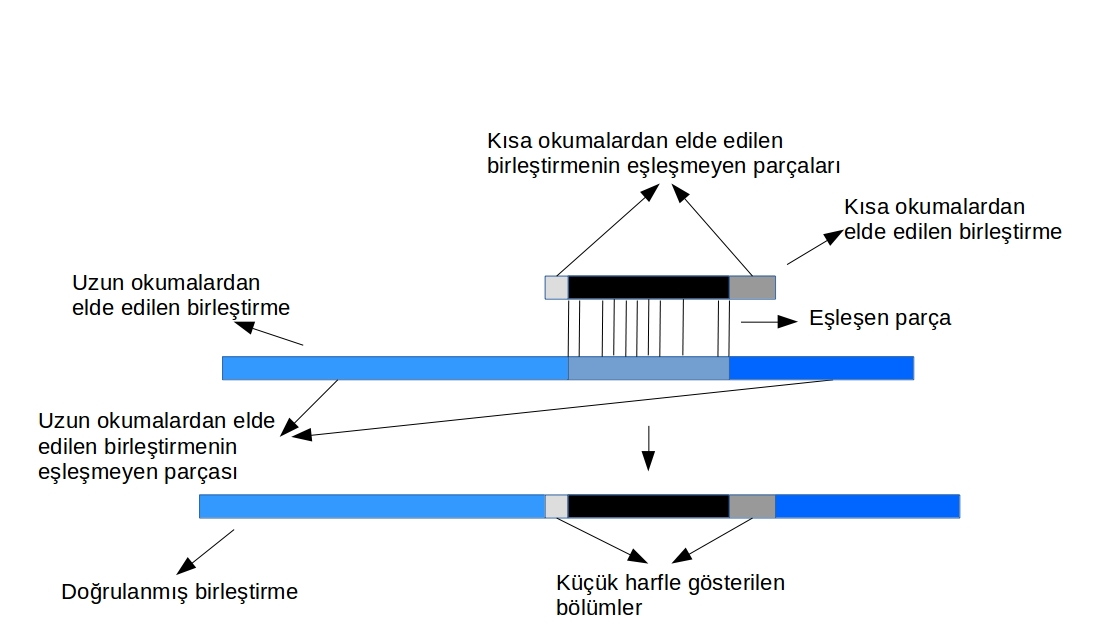
\includegraphics[width=14cm, height=8cm]{BACAlgorithmTurkce.jpg}
\end{center}
  \caption{Doğrulama metodu: Uzun okuma birleştirmelerini kısa okuma birleştirmelerinin hizalama bilgilerine göre doğrula.}
  \label{correction}
\end{figure}







